%%----------------------------------------------------------------------------
%% Presentatie HoGent Bedrijf en Organisatie
%%----------------------------------------------------------------------------
%% Auteur: Bert Van Vreckem [bert.vanvreckem@hogent.be]

\documentclass{beamer}

%==============================================================================
% Aanloop
%==============================================================================

%---------- Packages ----------------------------------------------------------

\usepackage{graphicx,multicol}
\usepackage{comment,enumerate,hyperref}
\usepackage{amsmath,amsfonts,amssymb}
\usepackage{tikz}
\usepackage[english]{babel}
\usepackage[utf8]{inputenc}
\usepackage{multirow}
\usepackage{eurosym}
\usepackage{listings}
\usepackage[T1]{fontenc}
\usepackage{lmodern}
\usepackage{textcomp}
\usepackage{framed}
\usepackage{wrapfig}
\usepackage{lstautogobble}

%---------- Configuratie ------------------------------------------------------

\usetikzlibrary{arrows,shapes,backgrounds,positioning,shadows}

\usetheme{hogent}

%---------- Commando-definities -----------------------------------------------
\definecolor{forestgreen}{RGB}{34,139,34}
\definecolor{orangered}{RGB}{239,134,64}
\definecolor{darkblue}{rgb}{0.0,0.0,0.6}
\definecolor{gray}{rgb}{0.4,0.4,0.4}
\newcommand{\tabitem}{~~\llap{\textbullet}~~}
\lstdefinestyle{java}{language=Java,
								backgroundcolor=\color{white},
								frame=single,
                basicstyle=\footnotesize\ttfamily,
                keywordstyle=\footnotesize\color{blue}\ttfamily,
								commentstyle=\color{forestgreen},
								breaklines=true,
								breakatwhitespace=true,
								tabsize=2,
								columns=fullflexible,
								autogobble=true,
								showstringspaces=false,
								showtabs=true,
}
\lstdefinestyle{XML}
{	basicstyle=\tiny\ttfamily,
  columns=fullflexible,
	frame=single,
  showstringspaces=false,
  commentstyle=\color{forestgreen}\upshape
  morestring=[b]",
  morestring=[s]{>}{<},
  morecomment=[s]{<?}{?>},
  stringstyle=\color{black},
  identifierstyle=\color{darkblue},
  keywordstyle=\color{forestgreen},
  morekeywords={xml,xmlns,version,type,android}% list your attributes here
}

%---------- Info over de presentatie ------------------------------------------

\title[Intro]{Quick Workshop Android}
\author{Dr. Jens Buysse }
\date{2014-2015}

%==============================================================================
% Inhoud presentatie
%==============================================================================

\begin{document}

%---------- Front matter ------------------------------------------------------

% Dia met het HoGent logo
\HoGentLogo

% Titeldia met faculteitslogo
\titleframe

%---------- Inhoud ------------------------------------------------------------

\section{Welcome to Mobile: Android}
\sectionframe

\begin{frame}
	\frametitle{Hello Android}
	I've come up with a set of rules that describe our reactions to
technologies:
\begin{enumerate}
	\item Anything that is in the world when you're born is normal and ordinary and is just a natural part of the way the world works.
	\item Anything that's invented between when you're fifteen and thirty-five is new and exciting and revolutionary and you can probably get a career in it.
	\item Anything invented after you're thirty-five is against the natural order of things.
\end{enumerate}
\begin{flushright}

\end{flushright}
-- Douglas Adams, author of \textsl{Hithhiker's Guide to the Galaxy}
\end{frame}

\begin{frame}
	\frametitle{Mobile Development}
	\begin{columns}
		\begin{column}{0.3 \textwidth}
		\pause
		\begin{figure}
			\centering
				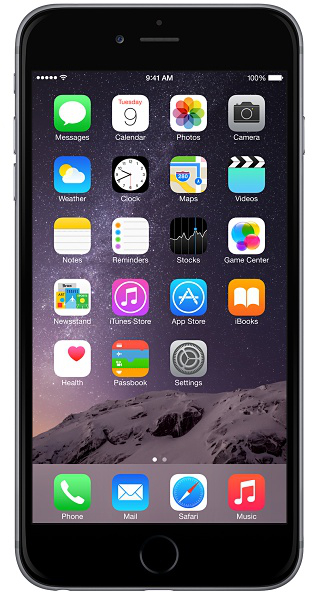
\includegraphics[width=1.00\textwidth]{img/iphone.jpg}
			\label{fig:iphone}
		\end{figure}
		
		\end{column}
		\begin{column}{0.3 \textwidth}
		\pause
			\begin{figure}
			\centering
				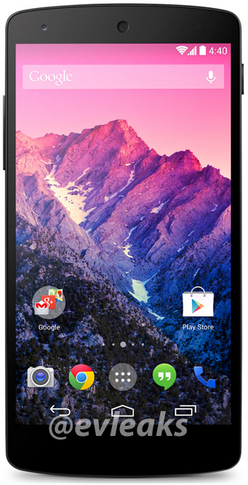
\includegraphics[width=1.00\textwidth]{img/nexus.png}
			\label{fig:iphone}
		\end{figure}
		\end{column}
		\begin{column}{0.3 \textwidth}
		\pause
			\begin{figure}
			\centering
				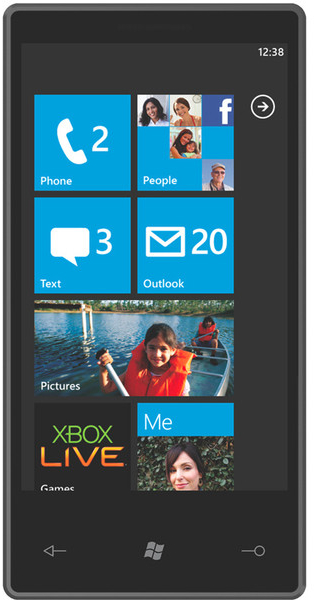
\includegraphics[width=1.00\textwidth]{img/windowsPhone.jpg}
			\label{fig:iphone}
		\end{figure}
		\end{column}
	\end{columns}
\end{frame}


{
\usebackgroundtemplate{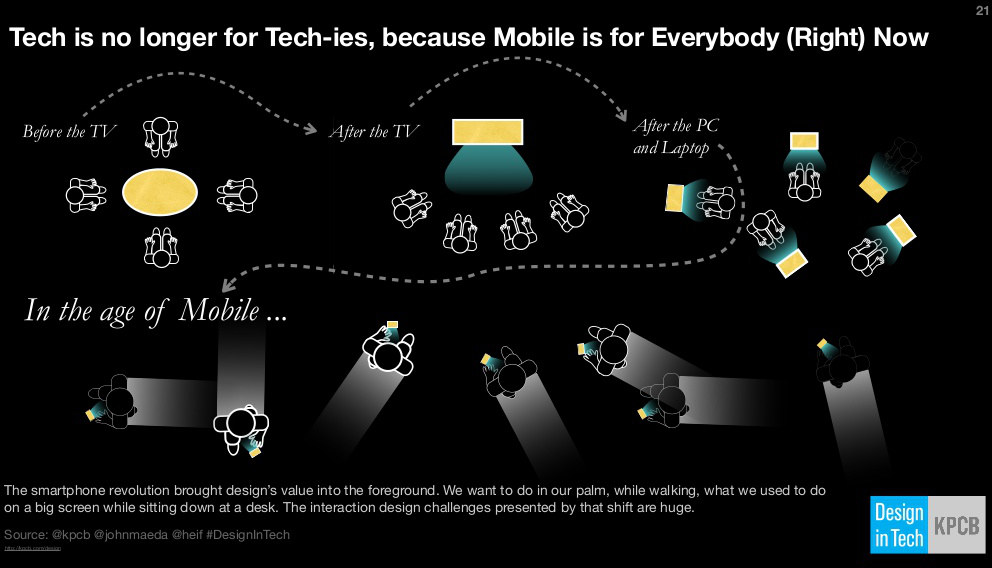
\includegraphics[height=\paperheight,width=\paperwidth]{img/timeLineMobile.jpg}}
\setbeamertemplate{navigation symbols}{}
\begin{frame}[plain]
\end{frame}
}

\begin{frame}
	\frametitle{What is Android}
	
	\begin{figure}
		\centering
			
\includegraphics[width=0.3 \textwidth]{img/androidlogo.png}
		\label{fig:androidlogo}
	\end{figure}
	
	Android is a ecosystem consisting of the following components:
	
	\begin{enumerate}
		\item A free, open source, operating system for embedded devices \pause
		\item An open source development platform to create mobile applications \pause
		\item Devices, specifically mobile devices, which run the mobile Android OS and the applications made for it
	\end{enumerate}
	 
	See \url{http://developer.android.com/training}
	
\end{frame}

{
	\usebackgroundtemplate{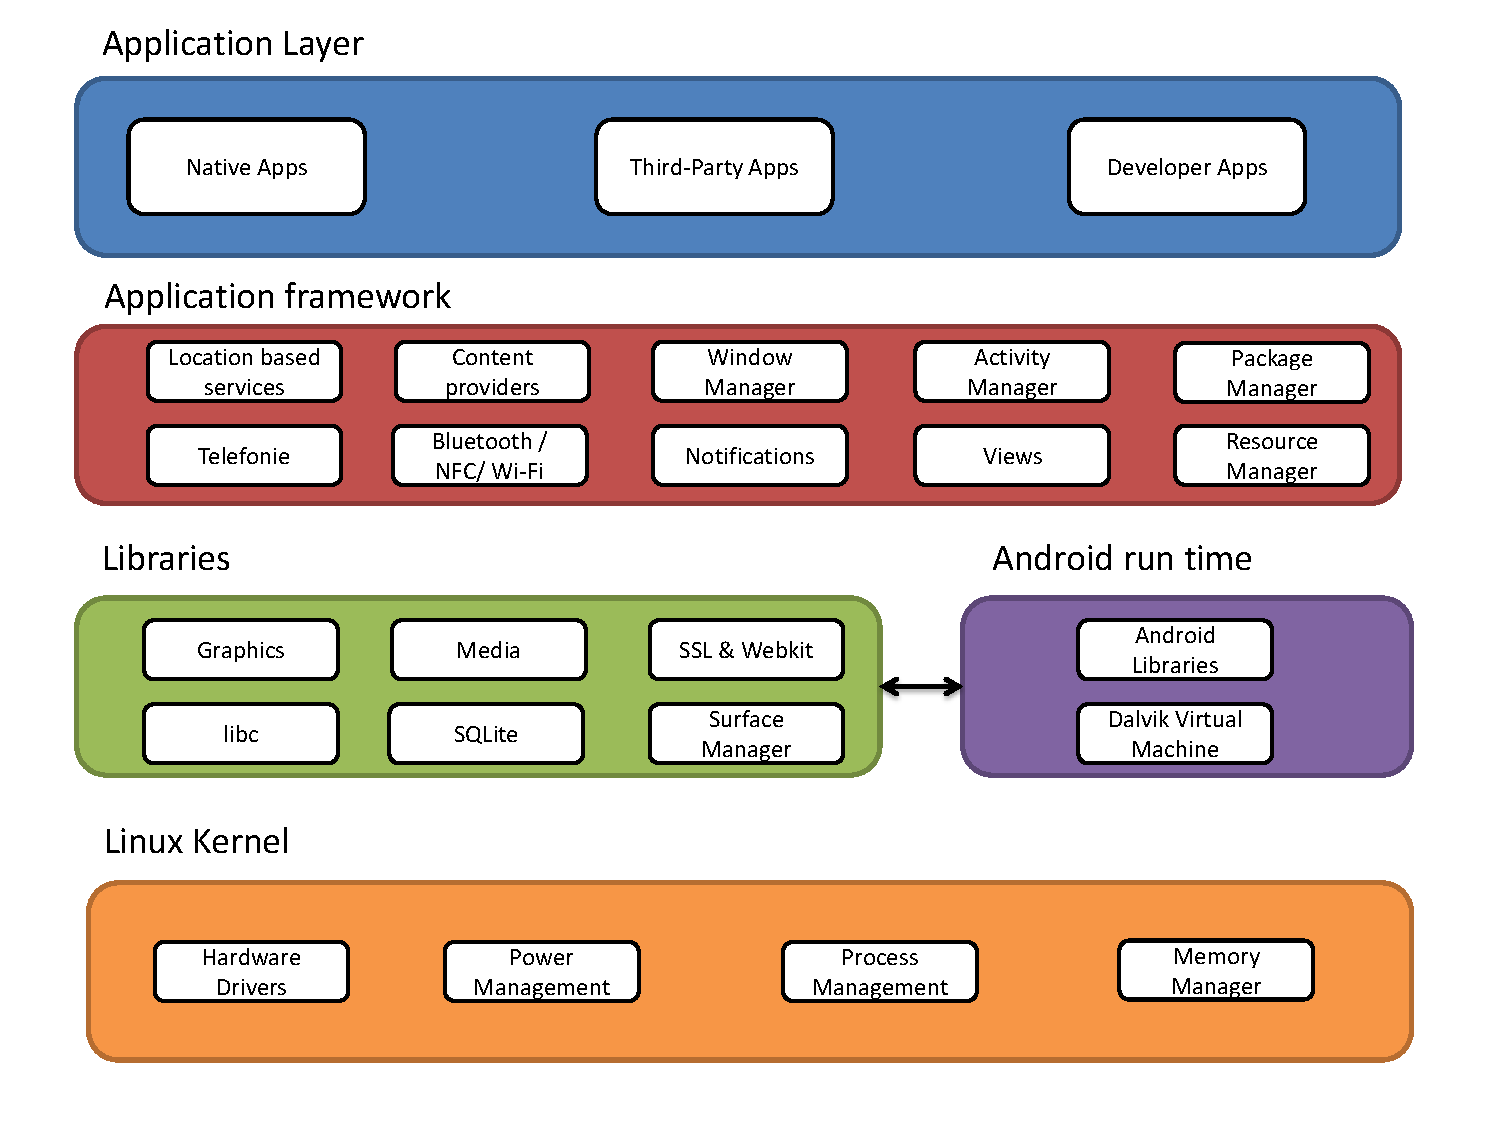
\includegraphics[height=\paperheight,width=\paperwidth]{img/androidstack.pdf}}
	\setbeamertemplate{navigation symbols}{}
	\begin{frame}[plain]
	\end{frame}
}
	
\begin{frame}
\frametitle{Linux Kernel}
Core services:
\begin{itemize}
\item Hardware drivers
\item Process and Memory management
\item Security and Power Management
\end{itemize}
De Kernel is a layer of abstraction between hardware and rest of Software Stack

\begin{figure}[b]
	\centering
		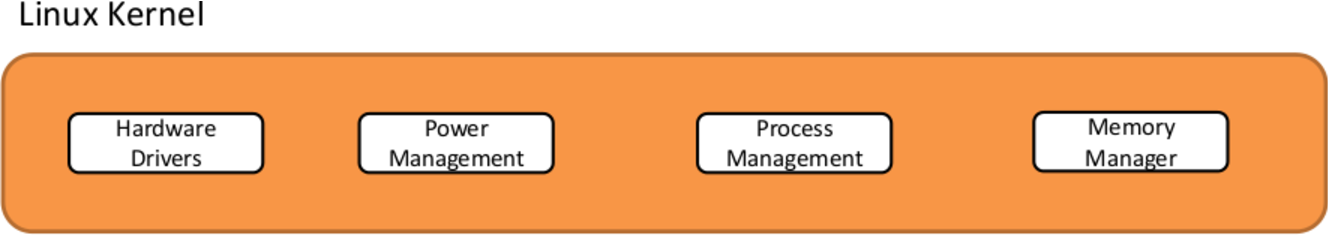
\includegraphics[width=\textwidth]{img/kernel.pdf}
	\label{fig:kernel}
\end{figure}

\end{frame}

\begin{frame}
\frametitle{Libraries}
\begin{itemize}
\item Media Library
\item Graphical libraries 
\item SQLLite for database support
\item \dots
\end{itemize}

\begin{figure}[b]
	\centering
		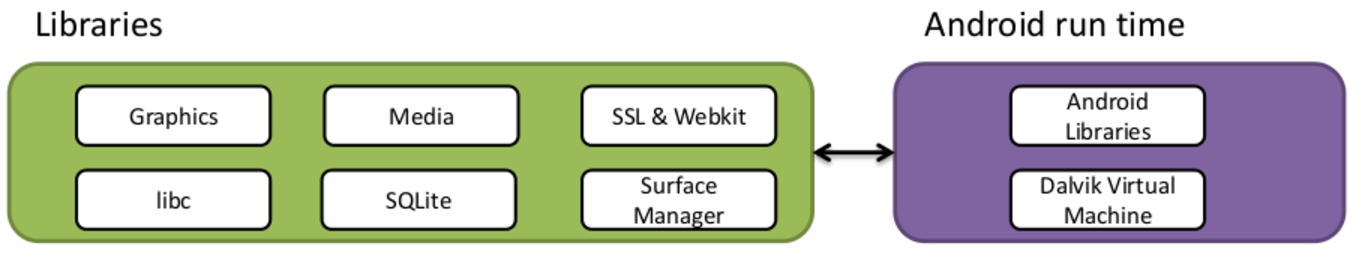
\includegraphics[width=\textwidth]{img/runtimeLibraries.pdf}
	\label{fig:kernel}
\end{figure}

\end{frame}

\begin{frame}
\frametitle{Run time}
\begin{itemize}
\item Core Libraries: proper implementations for the Dalvik Virtual Machine $\neq$ Java VM
\item Dalvik VM: virtual machine for Android, optimized for mobile devices (battery, processor \& memory management) 
\end{itemize}

\begin{figure}[b]
	\centering
		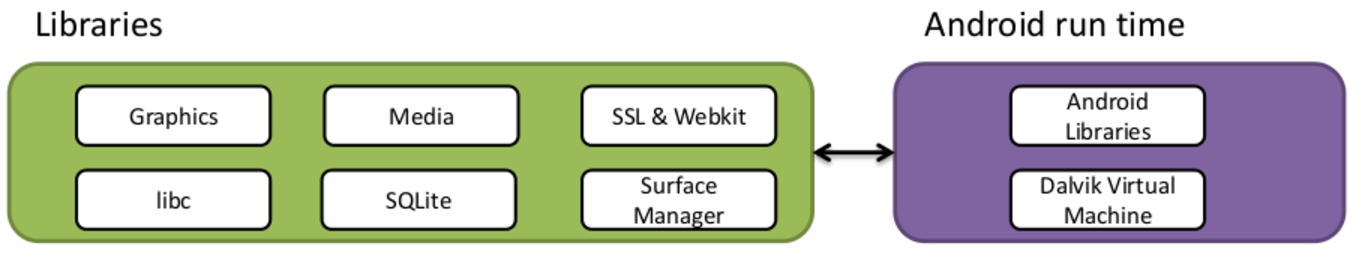
\includegraphics[width=\textwidth]{img/runtimeLibraries.pdf}
	\label{fig:kernel}
\end{figure}

\end{frame}

\begin{frame}
	\frametitle{Dalvik Virtual Machine}
	
	\begin{itemize}
		\item Typical Java VMs $\Rightarrow$ stack machines
		\item Dalvik VM $\Rightarrow$ a register-based architecture: cooler and thus uses less battery energy
		\item Each app uses its own process: sandboxing $\Rightarrow$ cornerstond of security in Android
	\end{itemize}
	\pause
	But \dots
	
	\begin{itemize}
		\item Android 5.0 \textit{Lollipop}: Dalvik was entirely replaced by \textsl{ART} (Android RunTime)
	\end{itemize}
\end{frame}

\begin{frame}
\frametitle{A typical work flow}

\begin{enumerate}
	\item App written in java
	\item Compiled to Java bytecode files
	\item dx converts java bytecode files to a single dex bytecodefile (classes.dex)
	\item Dalvik executes dex bytecode file 
\end{enumerate}
\end{frame}

\begin{frame}
\frametitle{Application Framework}
	The application framework provides the classes which can be used to create Android applications: an interface for access to the hardware 
	\begin{figure}[b]
	\centering
		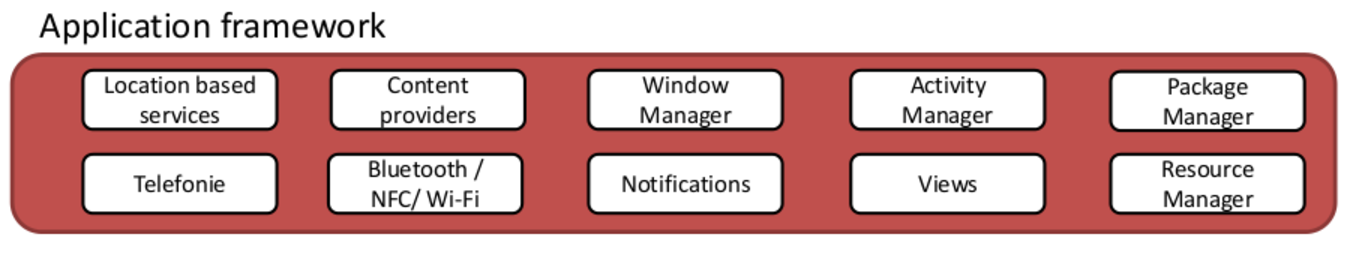
\includegraphics[width=\textwidth]{img/appFramework.pdf}
	\label{fig:kernel}
\end{figure}
\end{frame}

\begin{frame}
\frametitle{Application Layer}
	All applications are build in the application layer, using the different API libraries, and executed in the Dalvik VM. 
	\begin{figure}[b]
	\centering
		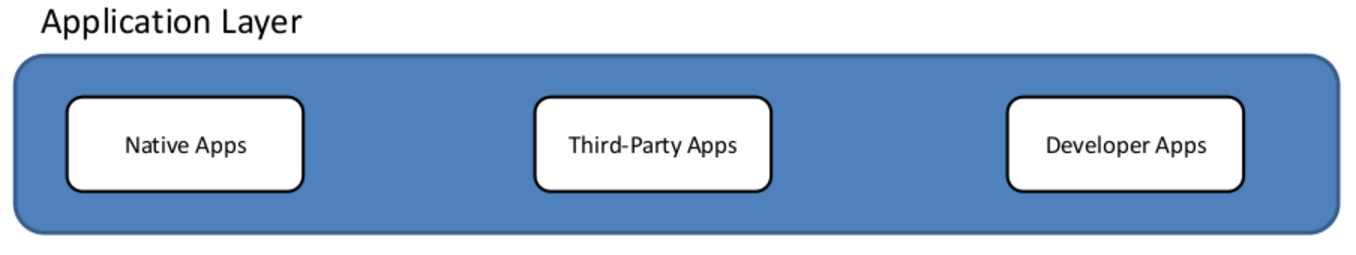
\includegraphics[width=\textwidth]{img/apllicationLayer.pdf}
	\label{fig:kernel}
\end{figure}
\end{frame}


{
	\usebackgroundtemplate{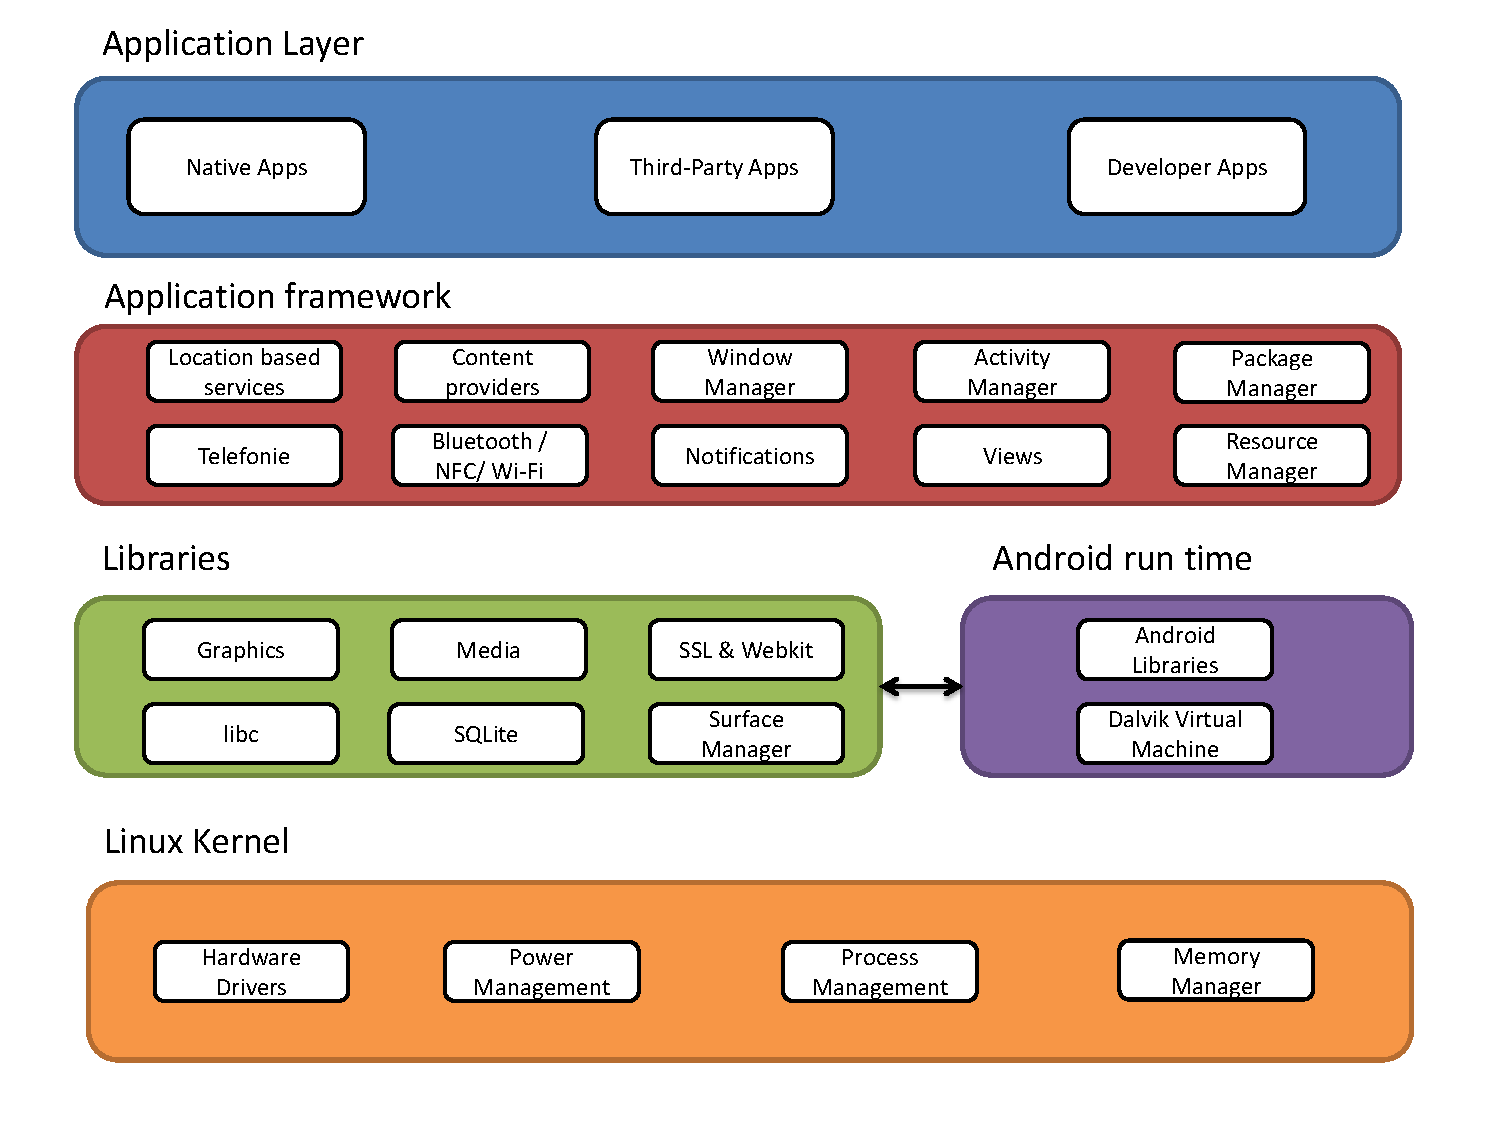
\includegraphics[height=\paperheight,width=\paperwidth]{img/androidstack.pdf}}
	\setbeamertemplate{navigation symbols}{}
	\begin{frame}[plain]
	\end{frame}
}




\section{Basic Programming in Android}
\sectionframe

\begin{frame}
\frametitle{Google is your friend!}
\begin{figure}
	\centering
		
\includegraphics[width=0.8\textwidth]{img/google.jpg}
	\label{fig:google}
\end{figure}
\begin{itemize}
	\item \url{http://developer.android.com/index.html}
	\item \url{http://android-developers.blogspot.be/}
	\item \dots
\end{itemize}
\end{frame}



\subsection{Activities \& Activity Lifecycle}

\begin{frame}
	\frametitle{Activities \& Activity Lifecycle}
	\brightbox{An \textcolor{HoGentAccent6}{Activity} is a single screen the user sees on the device at one time}
	
	\begin{figure}
		\centering
			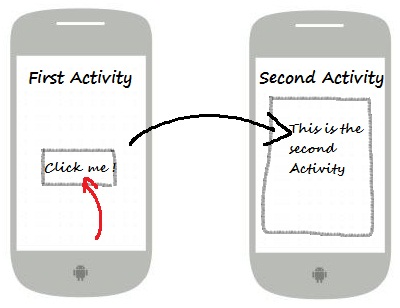
\includegraphics[width=0.6\textwidth]{img/activitySketch.jpg}
		\label{fig:activitySketch}
	\end{figure}
	\pause
	
	\begin{center}
	Comparable: www 
	\end{center}
\end{frame}

\begin{frame}
	\frametitle{Activity Life Cycle}
	The \textcolor{HoGentAccent6}{activity manager} is responsible for creating, destroying and managing activities. 
		\begin{columns}
			\begin{column}{0.4 \textwidth}
			
				\begin{figure}
					\centering
						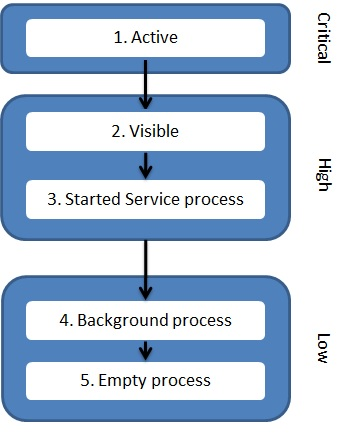
\includegraphics[width=\textwidth]{img/actState.jpg}
				\end{figure}
			
	\end{column}
	
	\begin{column}{0.6 \textwidth}
			
			\begin{itemize}
				\item \textbf{Active process}: have components which interact with the user
				\item \textbf{Visible process}: visisble but inactive process (e.g. non-full screen or transparant)
				\item \textbf{Started service process}: Process hosting and services
				\item \textbf{Background process}: process with non-visible activities and without started services
				\item \textbf{Empty process}: to improve memory management, apps are stored in memory 
			\end{itemize}
	\end{column}
	\end{columns}
\end{frame}

\begin{frame}
	\frametitle{De Activity Lifecylce}
	An acitivity has 4 states:
	
	\begin{description}
		\item [Running] is on top of the activity stack, is able to be manipulated and Android will do everything to keep this alive
		\item [Paused]  activity still visible, but interaction is not possible (e.g. when transparant)
		\item [Stopped] activity is invisible, but still in memory
		\item [Destroyed] activity is not on the stack any more and needs to be restarted
	\end{description}
\end{frame}


{
	\usebackgroundtemplate{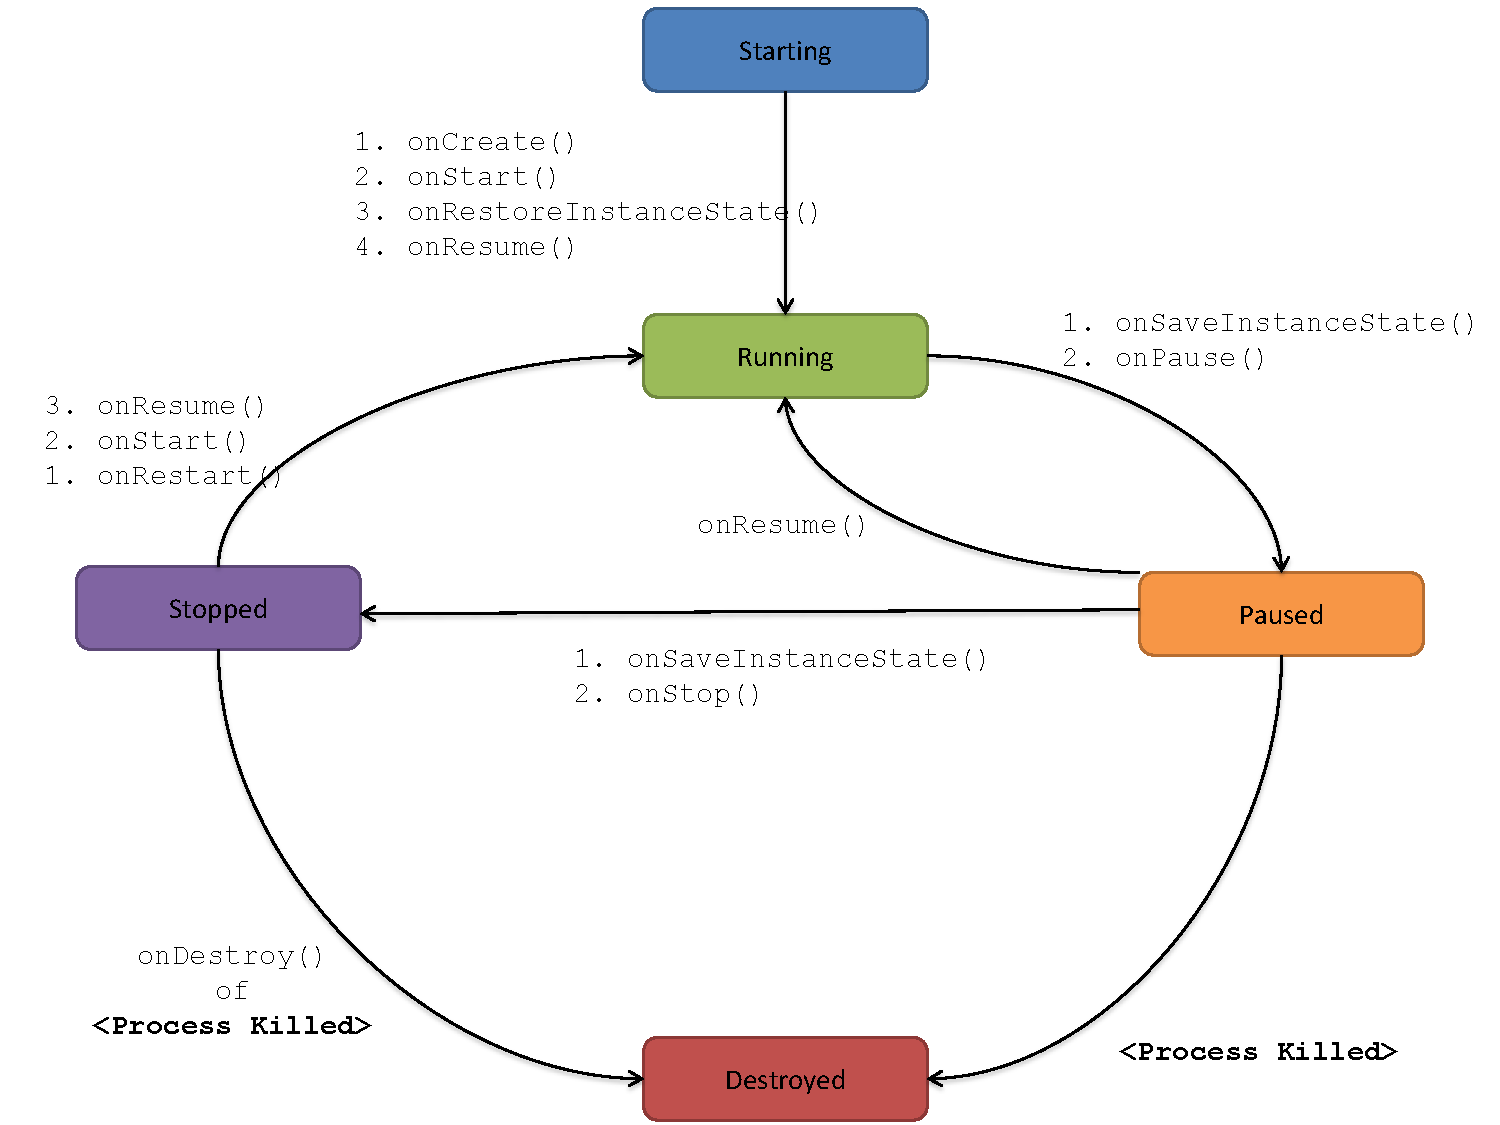
\includegraphics[height=\paperheight,width=\paperwidth]{img/activityLifeCycle.pdf}}
	\setbeamertemplate{navigation symbols}{}
	\begin{frame}[plain]
	\end{frame}
}

\subsection{Project layout}
\begin{frame}
	\frametitle{Anatomy Android Project }
	\begin{description}
		\item [Manifest File] Glues the project together (building blocks, permissions \dots)
		\item [String resources] \texttt{res/values/strings.xml} $\Rightarrow$ all the strings for the app
		\item [Layout XML colde] \texttt{res/layout/} declares the layouts of the activities
		\item [Drawable Resources] all images used in the app
		\item [R file] The connections between java and the external resources: automatically generated
		\item [Source Code]	the java source code for the app
	\end{description}
\end{frame}

\begin{frame}
	\frametitle{Emulator}
	
	\begin{itemize}
		\item The SDK comes with an emulator (lacks in performance though \dots )
		\item Genymotion is an emulator which is better
	\end{itemize}
\end{frame}

\begin{frame}
	\frametitle{Demonstration}
	See \url{https://github.com/eothein/Presentation-Android-Introduction}
\end{frame}

\section{Tutorial: lets go for it!}

\begin{frame}
	\frametitle{Goal of application}
	We will build an application which downloads a random Chuck Norris Joke and add this to a list
\end{frame}

\begin{frame}[fragile]
	\frametitle{Step 1: create the activity}
	
	\begin{itemize}
		\item Start a new project
		\item Choose to create a new Activity, lets call this MainActivity
		\item Create the layout (use LinearLayout and add a ListView and a Button)
		\item Do not forget to create the string constant for the button text
		\item You Should be able to start the application!
	\end{itemize}
	\pause
	Don't forget \dots
	\begin{lstlisting}[style=XML]
	 <uses-permission android:name="android.permission.INTERNET" />
	\end{lstlisting}
\end{frame}

\begin{frame}[fragile]
	\frametitle{Asynctask}
	\brightbox{An \textcolor{HoGentAccent6}{Asynctask} allows to perform background operations and publish results on the UI thread without having to manipulate threads and/or handlers.}
		\begin{lstlisting}[style=java]
			public void onClick(View v) {
    new DownloadImageTask().execute("http://example.com/image.png");
}

private class DownloadImageTask extends AsyncTask<String, Void, Bitmap> {
    /** Excutes in worker thread */
    protected Bitmap doInBackground(String... urls) {
        return loadImageFromNetwork(urls[0]);
    }
    
    /** Returns results */
    protected void onPostExecute(Bitmap result) {
        mImageView.setImageBitmap(result);
    }
}
		\end{lstlisting}
\end{frame}

\begin{frame}
	\frametitle{Asynctask}

\begin{description}
	\item [onPreExecute()]  used to setup the task
  \item [doInBackground(Params\dots)] invoked on the background thread immediately after onPreExecute() finishes executing. This step is used to perform background computation that can take a long time. 
    \item [onProgressUpdate(Progress \dots)], invoked on the UI thread after a call to publishProgress(Progress...) and used to display any form of progress in the user interface 
    \item [onPostExecute(Result)] invoked on the UI thread after the background computation finishes
\end{description}

\end{frame}

\begin{frame}
	\frametitle{Step 2: create an AsyncTask}
	Create the AsyncTask
	The three types used by an asynchronous task are the following:

\begin{description}
	\item [Params] the type of the parameters sent to the task upon execution.
  \item [Progress] the type of the progress units published during the background computation.
  \item [Result] the type of the result of the background computation.
\end{description}

\end{frame}

\begin{frame}
	\frametitle{Step 3: use GSON}
	In File $\rightarrow$ Project Structure $\rightarrow$ app $\rightarrow$ Dependencies add GSON 
\end{frame}

\begin{frame}[fragile]
	\brightbox{\textcolor{HoGentAccent6}{Gson} is a Java library that can be used to convert Java Objects into their JSON representation and vice versa}
	\begin{lstlisting}[style=java]
	class BagOfPrimitives {
  private int value1 = 1;
  private String value2 = "abc";
  private transient int value3 = 3;
  BagOfPrimitives() {
    // no-args constructor
  }
}
BagOfPrimitives obj = gson.fromJson(json, BagOfPrimitives.class);   
	
	\end{lstlisting}
\end{frame}

\begin{frame}
	\frametitle{Step 3: use GSON}
	
	\begin{itemize}
		\item Make a connection to \url{http://api.icndb.com/jokes/random?}
		\item Download the JSON response
		\item Use GSON to parse into a joke object
		\item In Mainactivty add a listener to the button and start the asynctask
		\item Test by logging to the logcat
	\end{itemize}
\end{frame}


\begin{frame}
	\frametitle{BroadcastReceivers and Intents}
	\brightbox{A \textcolor{HoGentAccent6}{broadcast receiver}  is an Android component which allows you to register for system or application events. All registered receivers for an event are notified by the Android runtime once this event happens. }
	
	
\end{frame}

{
	\usebackgroundtemplate{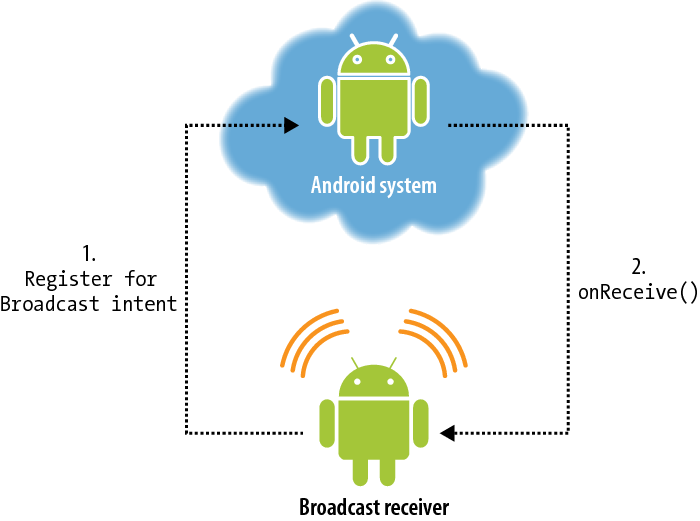
\includegraphics[height=\paperheight,width=\paperwidth]{img/broadcastReceiver.png}}
	\setbeamertemplate{navigation symbols}{}
	\begin{frame}[plain]
	\end{frame}
}

\begin{frame}
	\frametitle{Create a broadcastreceiver}
	
	\begin{itemize}
		\item Create the JokeReceiver
		\item Implements the onReceive methode
		\item Make an interface which the activity must implements (to add the joke)
		\item Create the intent and send it to the broadcastreceiver
	\end{itemize}
\end{frame}

\begin{frame}
	\frametitle{ListView and Adapter}
	
	\begin{figure}
		\centering
			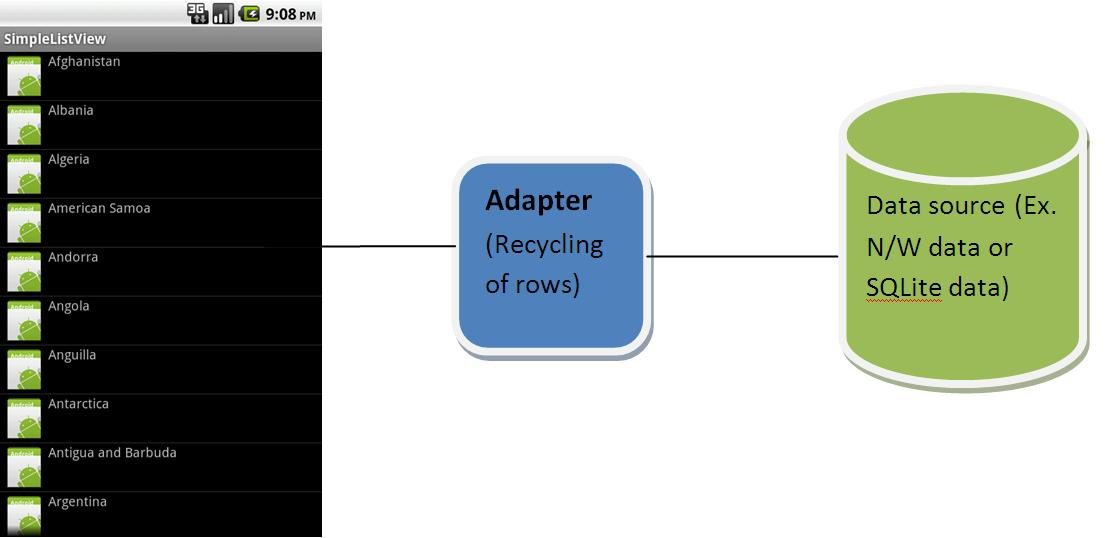
\includegraphics[width=1.00\textwidth]{img/adapter.jpg}
		\label{fig:adapter}
	\end{figure}
	
\end{frame}

\begin{frame}
	\frametitle{Create the adapter}
	
	\begin{itemize}
		\item Add an arraylist with strings in the activity
		\item Couple this with the arrayAdapter
		\item Allow to add strings to the list (implement the interface)
	\end{itemize}
\end{frame}


%---------- Back matter -------------------------------------------------------

\end{document}
